\documentclass[12pt]{article}

\usepackage{amsmath, amsfonts, amssymb}
\usepackage{graphicx}

\usepackage{epstopdf}

\newcommand{\SI}[0]{\textit{SI Materials and Methods}}

\begin{document}

\section{Introduction}

This is code for the registration and ordering algorithms described in \\
``Temporal ordering and registration of images in studies of developmental dynamics,'' Carmeline~J.~Dsilva, Bomyi~Lim, Hang~Lu, Amit~Singer , Stanislav~Y.~Shvartsman, and Ioannis~G.~Kevrekidis

The code reads in a set of two-dimensional images or three-dimensional z-stacks, can perform a number of preprocessing operations, and then registers and/or orders the images using the algorithms described in the paper. 

\section{Requirements}

All algorithms and analysis were implemented in MATLAB\textsuperscript{\textregistered} (R2013b, The MathWorks, Natick, Massachusetts).
%
The code requires MATLAB along with the Image Processing Toolbox. 

\section{How To Use}

There are two ways to use the code
\begin{enumerate}
\item Interactive GUI.
\item Program a simple script.
\end{enumerate}

The basic steps are as follows:
\begin{enumerate}
   \item Read in images
   \item Preprocess the images (smooth and/or equalize channels, mean-center, etc.)
   \item Run vector diffusion maps to register and order preprocessed images
   \item (Optional) Save registered and ordered images
   \item (Optional) Compute an average trajectory
\end{enumerate}

\subsection{Interactive GUI}

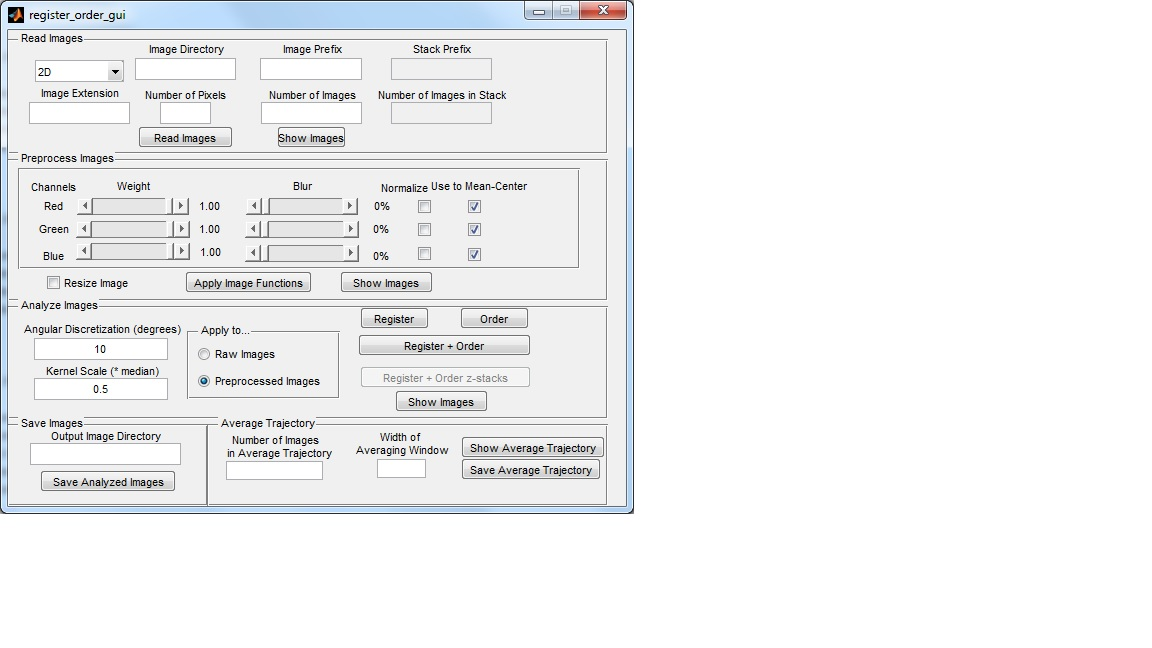
\includegraphics[width=\textwidth, trim=0cm 3cm 12cm 0cm, clip]{gui_screenshot_initial.jpg}

There are five steps
%
\begin{enumerate}
\item Read Images
\item Preprocess Images
\item Analyze Images
\item Save Images
\item Average Trajectory
\end{enumerate}

\subsubsection{Read Images}

The fields are as follows
\begin{description}
%
\item[2D/3D] Select ``2D'' if the images are traditional 2D images. Select ``3D'' if the images are z-stacks.
%
\item[Image Directory] Enter the directory where the images or z-stacks are stored. This directory can be an absolute path (e.g. \texttt{C:/Documents/Images}) or a path relative to the directory where this code is stored (e.g. \texttt{../Images})
%
\item[Image Prefix] The prefix for all image file names. The images are assumed to named as the image prefix, followed by a number. 
%
\item[Stack Prefix] (only for 3D z-stacks) The prefix for all stack folder names. Each stack is assumed to be stored in a single folder, with the folder's name as the stack prefix, followed by a number. 
%
\item[Image Extension] The extension of the images (e.g., tif, jpg)
%
\item[Number of Images] The number of images or z-stacks. Images are assumed to be stored as the image prefix, followed by a two-digit index, where the indices run from 1 to the number of images (e.g., image\_prefix01.tif, image\_prefix02.tif, etc.). For three-dimensional images, the z-stacks are assumed to be stored in individual folders whose names are the stack prefix, followed by a two-digit index, where the indices run from 1 to the number of stacks (e.g., z\_stack\_prefix01/, z\_stack\_prefix02/, etc.)
%
\item[Number of Images in Stack] (only for z-stacks) The number of images per z-stack. Images are assumed to be stored in the individual stack directories as the stack prefix, followed by a two-digit index, where the indices run from 1 to the number of images in the stack (e.g., stack\_prefix01.tif, stack\_prefix02.tif, etc.). 
%
\end{description}

After populating the required fields, select the ``Read Images'' button to read in the images.
%
After reading the images, (optional) select the ``Show Images'' button to display the images (z-stacks will be displayed as maximum intensity projections).

\subsubsection{Preprocess Images}

\begin{description}
\item[Weight] Each channel in the images is scaled by the weight factor, where all weights at 1 does not adjust the channel intensities. For grayscale images, only the first weight is used. 
%
\item[Blur] Each channel in the images is blurred using a disc factor with radius equal to a fraction of the image as indicated by the ``blur'' field. For example, setting the blur to 5\% means that the image is blurred using a disc filter with radius $0.05 \times$ the number of pixels. 
%
\item[Normalize] If the normalize option is selected for a specific channel, then Contrast-Limited Adaptive Histogram Equalization is applied to that channel to normalize the intensities across the image. This is important for signals whose absolute intensity is not meaningful or informative. 
%
\item[Use to Mean-Center] If the mean-center option is selected for any of the channels, then the object is centered in the image by detecting the edges of the object given by the selected channels. If no mean-center options are selected, then the object is not mean-centered.
%
\item[Resize Images] If the resize images option is selected, then each image is scaled/dialated so that the object occupies 80\% of the total image frame. This removes any size effects/variations in the images. 
%
\item[Number of Pixels] The number of pixels wanted in the images for analysis. This does {\em not} have to be the same number of pixels as the true resolution of the images. The images are assumed to be square. 
%
\end{description}

After populating the required fields, select the ``Apply Image'' button to apply the selected preprocessing options.
%
After preprocessing the images, (optional) select the ``Show Images'' button to display the preprocessed images (z-stacks will be displayed as maximum intensity projections).

\subsubsection{Analyze Images}

After preprocessing the images, one can apply various analysis algorithms. 
%
There are three parameters
%
\begin{description}
%
\item[Angular Discretization (degrees)] (required for image registration) This is the angular discretization used to search for the pairwise alignments between images. For example, if the angular discretization is 10$^\circ$, then the pairwise alignments are computed by computing the image discrepancy after 10$^\circ$ rotation, after a 20$^\circ$ rotation, ..., up to a 360$^\circ$ rotation, and then selecting the rotation which minimizes the discrepancy. Lower values of the angular discretization increase the accuracy of the method, but also increase the computational cost. 
%
\item[Kernel Scale (*median)] This is the scaling of the diffusion maps kernel, in multiples of the median of the pairwise distances (so that $\epsilon$ in the diffusion maps algorithm, as outlined in \SI, is this value times the median of the pairwise distances). This parameter should be $\mathcal{O}(1)$; empirically, we have found that values of $0.25-0.5$ often yield good results for our data sets. 
%
\item[Apply to...]  This determines which images are shown and/or saved as the analyzed images. Select the ``Apply to Raw Images'' option to apply the computed registration and/or ordering to the original images; select the ``Apply to Preprocessed Images'' option to apply the computed registration and/or ordering to the preprocessed images (after blurring, normalization, etc.)
%
\end{description}

There are four analysis options
\begin{description}
%
\item[Register] (this option is only for two-dimensional images) This registers the imaging data set using vector diffusion maps to compute the optimal rotations. 
%
\item[Order] This orders the imaging data set using diffusion maps. {\em Important:} This option assumes that the imaging data set is preregistered! This option is intended for imaging data sets that were preregistered using some {\em a priori} knowledge about the system. 
%
\item[Register + Order] (this option is only for two-dimensional images) This registers and orders the imaging data set using vector diffusion maps to compute the optimal rotations and the temporal ordering. 
%
\item[Register + Order z-stacks] (this option is only for three-dimensional z-stacks) This registers and orders the imaging data set. It first registers the z-stacks by computing the optimal rotations to align the (two-dimensional) maximum intensity projections using vector diffusion maps.  It then orders the data using diffusion maps on the (now registered) three-dimensional z-stacks. 
%
\end{description}

(Optional) After analysis select the ``Show Images'' button to display the registered and/or images (z-stacks will be displayed as maximum intensity projections). 


\subsubsection{Save Images}

This is the (optional) step of saving the analyzed images.
%
The ``Output Image Directory'' is where the analyzed images will be stored; this directory will be created if it does not exist. 
%
The images will be stored in the output directory, and the name format will be the same as in the input directory. 

\subsubsection{Average Trajectory}

An (optional) step is to compute the average trajectory of the registered and ordered images.

There are two parameters
\begin{description}
\item[Number of Images in Average Trajectory] This is the desired number of images in the average trajectory. 
%
\item[Width of Averaging Window] This is the (approximate) width of the averaging window. Each snapshot in the average trajectory will be the (weighted) average of approximately the width number of images (see \SI). Increasing this value will result in a smoother average trajectory, while decreasing this value will retain more finer-scale detail. 
% 
\end{description}

The ``Show Average Trajectory'' option will then display the average trajectory images. 
%
The ``Save Average Trajectory'' option will save the average trajectory images. 
%
The images will be saved in the ''Output Image Directory'' folder. 
%
The name format will be the same as the input file format, but with the prefix ``avg\_''.

\subsection{Script}

\subsection*{Read Images}

\begin{par}
The first step is to read in images. This is done using the \texttt{read\_images} function For two-dimensional images, it requires that all the images are stored in a single directory, all with a consistent prefix, and indexed with two digits starting from \texttt{01}. For three-dimensional z-stack, it assumes each z-stack is stored in a single directory. All of the z-stack directories are required to begin with a consistent prefix, and be indexed with two digits starting from \texttt{01}. Similarly, all of the images are required to begin with a consistent prefix, and be indexed with two digits starting from \texttt{01} for each z-stack.
\end{par} \vspace{1em}
\begin{verbatim}
% directory where images are stored
image_dir = 'drosophila_fixed_images';

% prefix for each image
image_name = 'emb';

% image type/extension
image_ext = 'tif';

% no stack name or number of iamges in a stack are required for 2D images
stack_name = '';
nstack = 0;

% number of images
nimages = 120;

% number of pixels
npixels = 100;

% dimension of images (dim=2 indicates standard 2D images, rather than
% z-stacks)
dim = 2;

% read in images
% images are stored in the variable images_raw
[images_raw, nchannels] = read_images(image_dir, image_name, image_ext, ...
    stack_name, nimages, nstack, npixels, dim);
\end{verbatim}


\subsection*{Show images}

\begin{par}
An optional step is to now show the images using the \texttt{plot\_images} function.
\end{par} \vspace{1em}
\begin{verbatim}
% plot the images
% images_raw are the images to plot
% (returned from the read_images function)
% dim is the dimension of the images
% (dim=2 indicates standard 2D images, rather than z-stacks)
plot_images(images_raw, dim)
\end{verbatim}

\includegraphics [width=4in]{sample_input_file_01.eps}


\subsection*{Preprocess Images}

\begin{par}
Now, we must preprocess the images before registration and ordering, to remove any imaging and/or experimental artifacts. We do this via the \texttt{apply\_image\_functions} function For this particular imaging data set, there are three channels. DAPI, a nuclear stain, is in the first (red) channel. dpERK is in the second (green) channel. Dl is in the third (blue) channel.
\end{par} \vspace{1em}
\begin{verbatim}
% channel weights
% because the nuclear signal is wider spread throughout the image, as well
% as noiser, we choose to scale the first channel by half
channel_weight = [0.5 1 1];

% we blur the image slightly (5%) so that small-scale effects of individual
% nuclei are smoothened
channel_blur = [0.05 0.05 0.05];

% because the absolute intensity of the nuclear signal is not informative
% or important (only the presence or absence of signal is important,
% indicating the presence or absence of nuclei), we normalize the first channel
% We do not normalize the other two channels, as changes in intensity are
% informative to the developmental processes.
channel_normalize = [1 0 0];

% we use the nuclear channel to mean center the images, as this channel
% parameterizes/captures the entire embryo
channel_mean_center = [1 0 0];

% we resize the images to all be (approximately) the same size, to remove
% any variations due to size effects, as size effects are known to not be
% important for this developmental system
resize_image = true;

% we then apply these image functions of normalization, blurring,
% reweighting, and mean-centering
images = apply_image_functions(images_raw, dim, channel_weight, ...
    channel_blur, channel_normalize, channel_mean_center, resize_image);

% plot the images (optional)
plot_images(images, dim)
\end{verbatim}

\includegraphics [width=4in]{sample_input_file_02.eps}


\subsection*{Calculate pairwise alignments}

\begin{par}
We now need to calculate the angles needed to align \textit{pairs} of images
\end{par} \vspace{1em}
\begin{verbatim}
% angular discretization when computing pairwise aligments
% this means we search for pairwise aligmemnts over 10 degree increments
ang_dis = 10;

% compute the pairwise alignments
% images are the preprocessed images
% ang_dis is the angular discretization
% R and W store the pairwise alignments and distances, respectively, for
% vector diffusion maps
[R, W] = compute_pairwise_alignments(images, ang_dis);
\end{verbatim}


\subsection*{Apply vector diffusion maps}

\begin{par}
We can now use vector diffusion maps to register and order the images.
\end{par} \vspace{1em}
\begin{verbatim}
% ncomps is the number of components to compute
% we only compute 1 coordinate because we only need to order the images
% (i.e., sort by the first coordinate)
ncomps = 1;

% epsilon scale for diffusion maps kernel
% eps_scale = 0.25 means that the epsilon in the diffusion maps kernel is
% 1/4 of the median of the pairwise distances between data points
eps_scale = 0.25;

% vector diffusion maps calculates optimal rotations and embedding
% coordinate
[R_opt, embed_coord, D2] = vdm(R, W, eps_scale, ncomps);

% register images
images_registered = register_all_images(images, R_opt);

% order registered images by embedding coordinate
images_analyzed = order_all_images(images_registered, embed_coord);

% plot the images (optional)
plot_images(images_analyzed, dim)
\end{verbatim}

\includegraphics [width=4in]{sample_input_file_03.eps}


\end{document}

